\subsection{Active Object}

The Active Object design pattern aims to enhance concurrency in a multi-threaded
distributed system. Much different from \textit{passive objects}, which execute
a method in the same thread of control in which it was invoked, active objects
separate these two mechanisms. Douglas Schmidt describes:

\begin{quote}
``\ldots the Active Object pattern decouples method execution from method
invocation in order to simplify synchronized access to an object that resides in
its own thread of control.'' \cite{Schmidt96}
\end{quote}

The Active Object design pattern operates under the principles that (1) methods
invoked on an object should not block, (2) synchronized access to shared objects
should be simple, and (3) applications should leverage the parallelism available
on the platform \cite{Schmidt96}. If an application needs access to some
service, but either the results do not matter or they do not matter immediately,
then invoking distributed operations should not be a blocking call.
Additionally, these operations should be interfaced and implemented on the
operating system's native networking layers so that using them is simple and
easy.

\begin{figure}[t]
  \begin{center}
  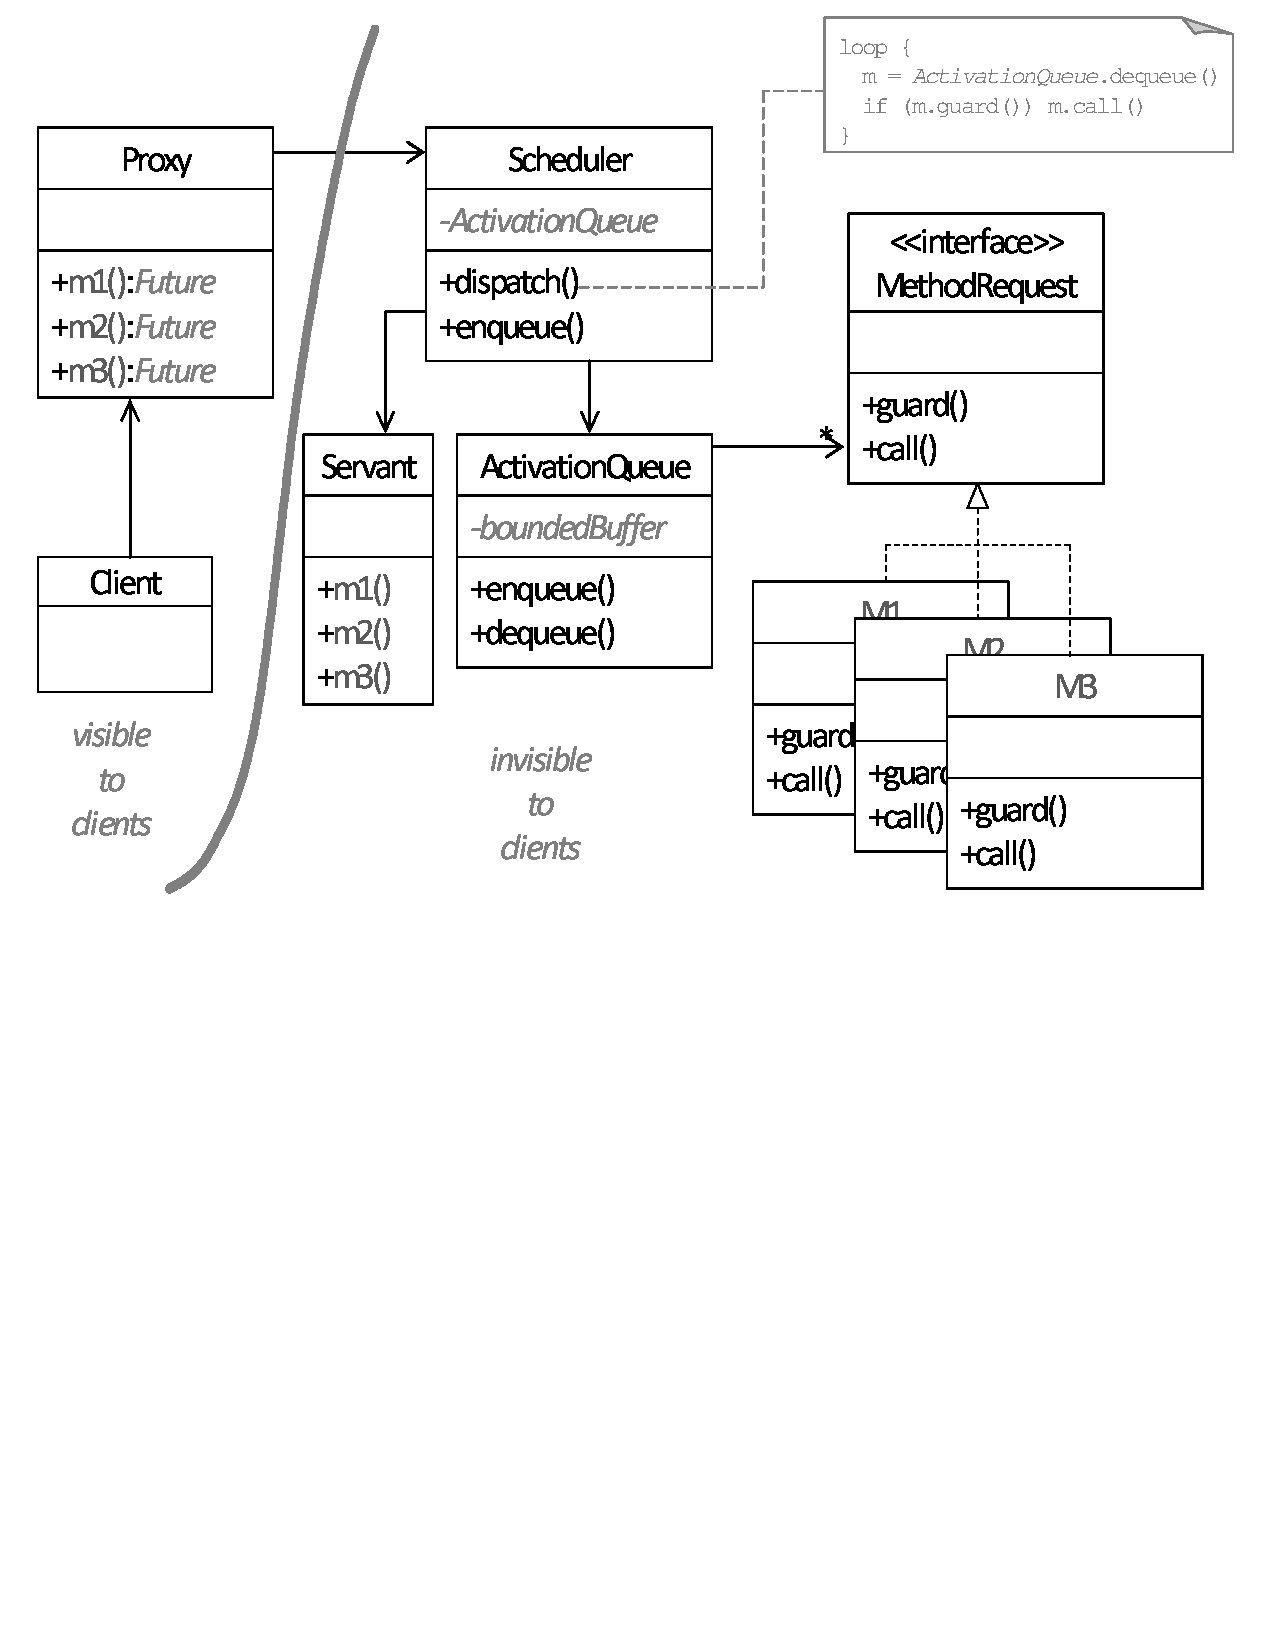
\includegraphics[width=\textwidth]{images/activeObjectUML}
  \caption{Active Object UML Diagram}
  \label{fig:activeObjectUML}
  \end{center}
\end{figure}

Recall that there are two primary components that make up the Active Object
design pattern: the \textbf{Proxy} and the \textbf{Scheduler}. The structure of
this pattern is illustrated in Figure \ref{fig:activeObjectUML}. The Active
Object design pattern is described in greater detail in \cite{Schmidt96}.

The components in this diagram are separated into two distinct threads of
control: one visible to clients and one invisible to clients. In general, the
Proxy object is responsible for providing an interface compliant with the target
object for the client. The scheduler, which resides in its own thread of
control, manages a queue method requests and decides which method to dequeue
and execute. The sequence diagram in Figure \ref{fig:activeObjectSequence}
illustrates the general flow of control. Again, the sequence diagram
separates the two separate threads of control: the thread in the client and the
thread in the service.

\begin{figure}[t]
  \begin{center}
  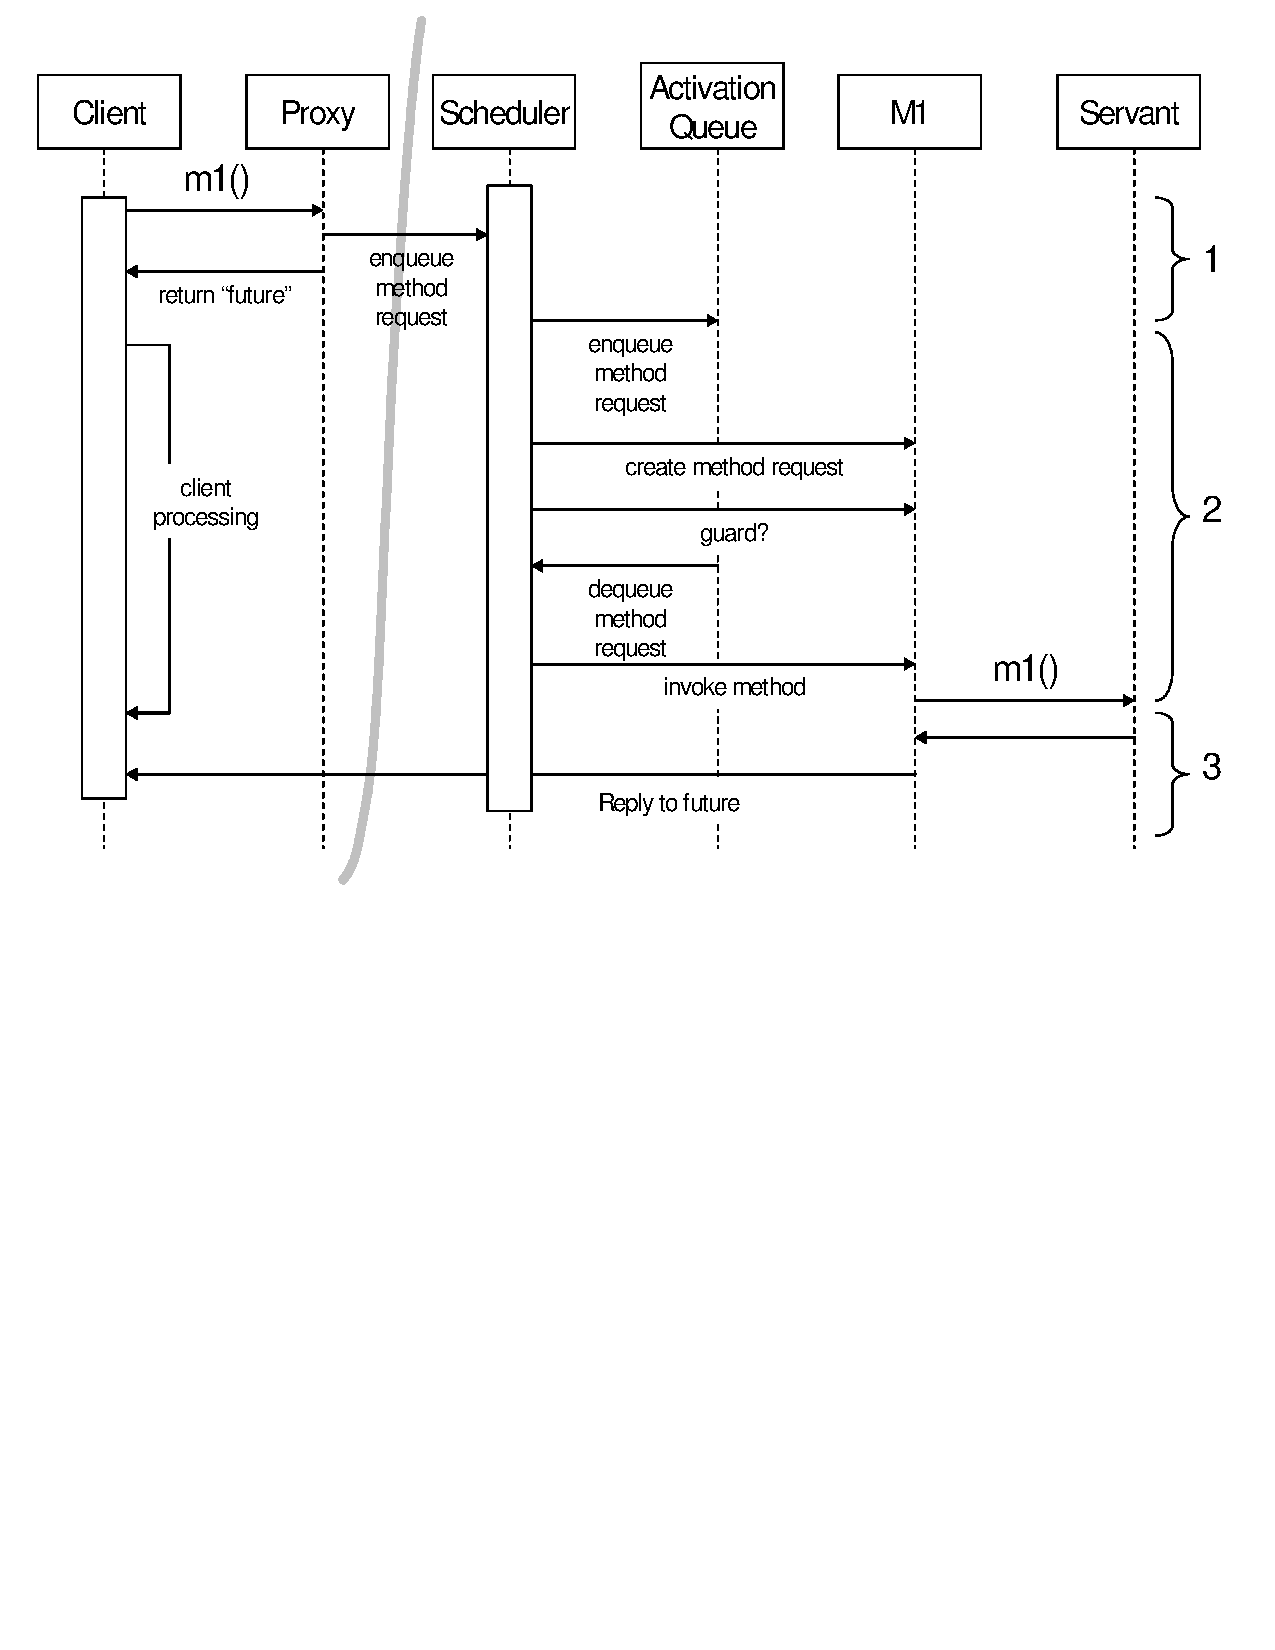
\includegraphics[width=\textwidth]{images/activeObjectSequence}
  \caption{Active Object Sequence Diagram}
  \label{fig:activeObjectSequence}
  \end{center}
\end{figure}

First, the client uses the proxy to invoke some method. This asynchronous  
request returns immediately with some ``future'' object that will store the
eventual result so the client can continue processing other tasks. The proxy
then connects to the scheduler, which will queue up the method request in the
activation queue. When the scheduler decides that the method is ready to be
dequeued, it will first check the guard on the method object to ensure that the
method itself is ready. It then invokes the method on the method object
instance, which invokes the method on the target object. The servant will return
the result and update the data in the future object which the client holds a
reference to.

\subsubsection{Active Object in Coursebook}

\begin{figure}[t]
\singlespacing
\makebox[\textwidth]{\hrulefill}
\begin{lstlisting}
String server  = ``http://api.facebook.com/restserver.php'';
String api_key = ``092fedbd6b45aae9db3febd6e96ee5e5'';
String secret  = ``f482a1bfff345991e9ff792771805741'';

FacebookRestClient client = 
  new FacebookRestClient(server, null, api_key, secret);

Document doc = client.callMethod(``facebook.auth.getSession'');
doc = client.callMethod(``facebook.users.getInfo'');
...
NodeList nodes = doc.getFirstChild().getChildNodes();
nodes = nodes.item(0).getChildNodes();
...
for (Node n: nodes)
{
  /* retrieve data from XML nodes */
}
\end{lstlisting}
\makebox[\textwidth]{\hrulefill}
\doublespacing
\caption{REST Code in Coursebook}
\label{fig:REST_code}
\end{figure}

In Coursebook, we use the Active Object design pattern, namely the Proxy 
component, to communicate with the different distributed modules of our system.
For example, Coursebook consists of several disparate services including a MySQL
Database, the WordNet API, and Facebook web services. We will discuss how
Coursebook exemplifies the Active Object design pattern through its use of the
Facebook REST service.

REST, or Representational State Transfer, is a simple stateless, cacheable,
client/server architectural style for distributed hypermedia systems 
\cite{Fielding00}. The goal of REST is to minimize latency and network
communication while maximizing independence and scalability of component 
implementations by transmitting domain specific data over HTTP without
additional messaging layers like SOAP or session tracking with cookies. You can
think of REST as a simple request-response system, essentially HTTP. In fact,
Roy Fielding, one of the primary architects of HTTP, designed REST in his
doctoral dissertation \cite{Fielding00}.

\begin{figure}[t]
  \begin{center}
  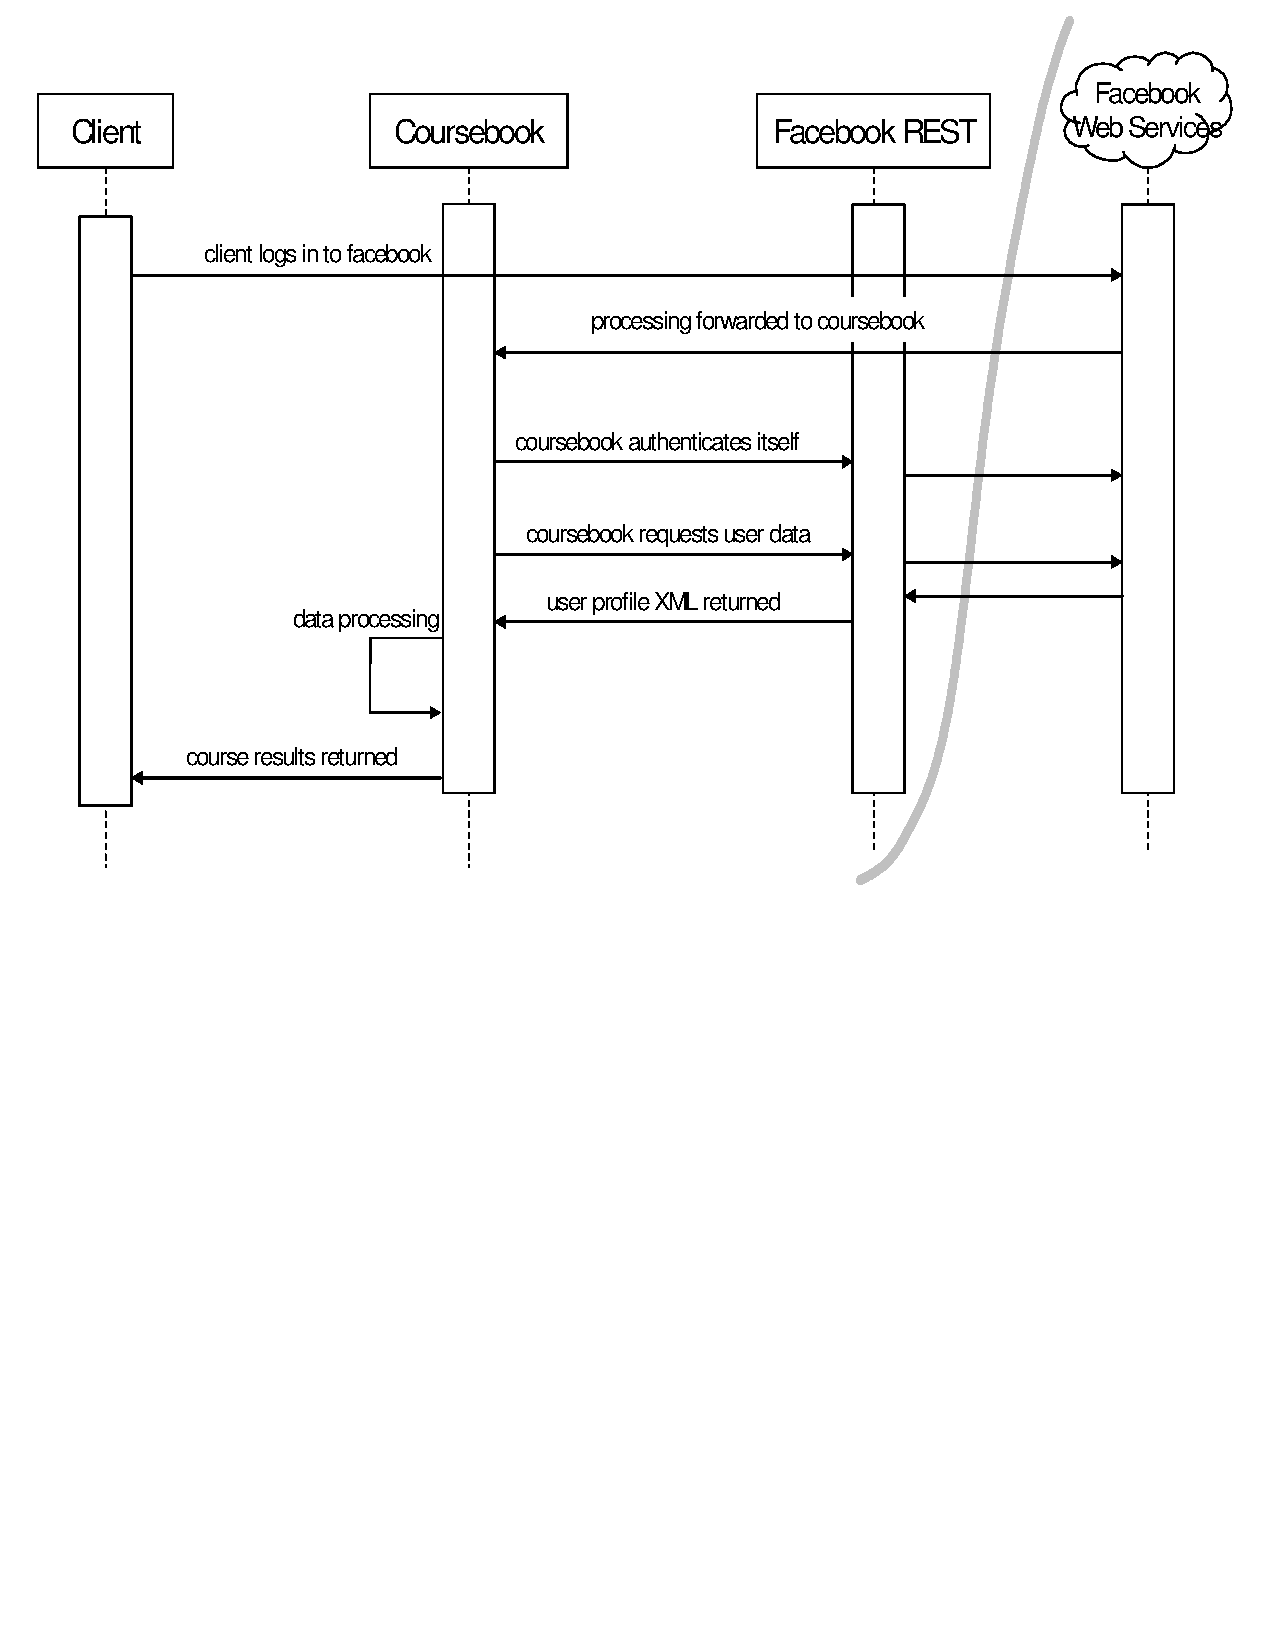
\includegraphics[width=\textwidth]{images/courseBookSequence}
  \caption{REST Web Service Sequence Diagram}
  \label{fig:courseBookSequence}
  \end{center}
\end{figure}

The Facebook API uses REST to service requests from web developers
\cite{Facebook}. The code listing in Figure \ref{fig:REST_code} shows a sample
of the tasks performed in our \verb!FacebookController!. In reference to the
Active Object design pattern, the \verb!FacebookController! behaves like the
client calling code and the \verb!FacebookRestClient! behaves as the proxy
object. Scheduling and actual method execution is handled in the Facebook Web
Service.

The sequence diagram shown in Figure \ref{fig:courseBookSequence} shows how
Coursebook uses the Facebook Web Service API in an Active Object manner. First,
a client using a web browser logs into the Facebook web site. The Facebook
developer web site will forward the user to the \verb!FacebookController! in
Coursebook. The controller uses the \verb!FacebookRestClient! object to invoke
methods like \verb!facebook.auth.getSession! and \verb!facebook.users.getInfo!.
These method requests are sent to the proxy, which are in turn sent to the
actual web service. Our controller continues to process until the the XML data
is returned from the web service. Once Coursebook has this data, it can finish
servicing the client's request.
